\documentclass[../main.tex]{subfiles}

\begin{document}

    \chapter{Name of chapter 4}
    %Bare for å generere noe tekst for å se hvordan det ser ut:
    \lipsum[1]
    
    \section{Name of section 1}
    %Bare for å generere noe tekst for å se hvordan det ser ut:
    \lipsum[1]\\
    It can be applied in this way \citep{example_reference1}. \\ \\
    A more detailed description is found in \autoref{tab:example_table1}. 
    
    \begin{table}[H]
        \small
        \caption{Example table 1.}
        \label{tab:example_table1}
        \centering
        \renewcommand{\arraystretch}{1.5}
        \begin{tabular}{l|p{25em}}
        \cellcolor{gray!25}Security level & \cellcolor{gray!25}Description \\
        \Xhline{2\arrayrulewidth}
            0 & The number 0\\
            \hline
            1 & The number 1\\
            \hline
            2 & The number 2 \\
            \hline
            3 & The number 3 \\
            \hline
            4 & The number 4 \\
            \hline
        \end{tabular}
        \renewcommand{\arraystretch}{1}
    \end{table}
    \color{black}
    
    %Bare for å generere noe tekst for å se hvordan det ser ut:
    \lipsum[1]\\
    A more detailed structure is shown in \autoref{fig:example_figure_2}.\\ \\
    
    \begin{figure}[H]
    \centering
    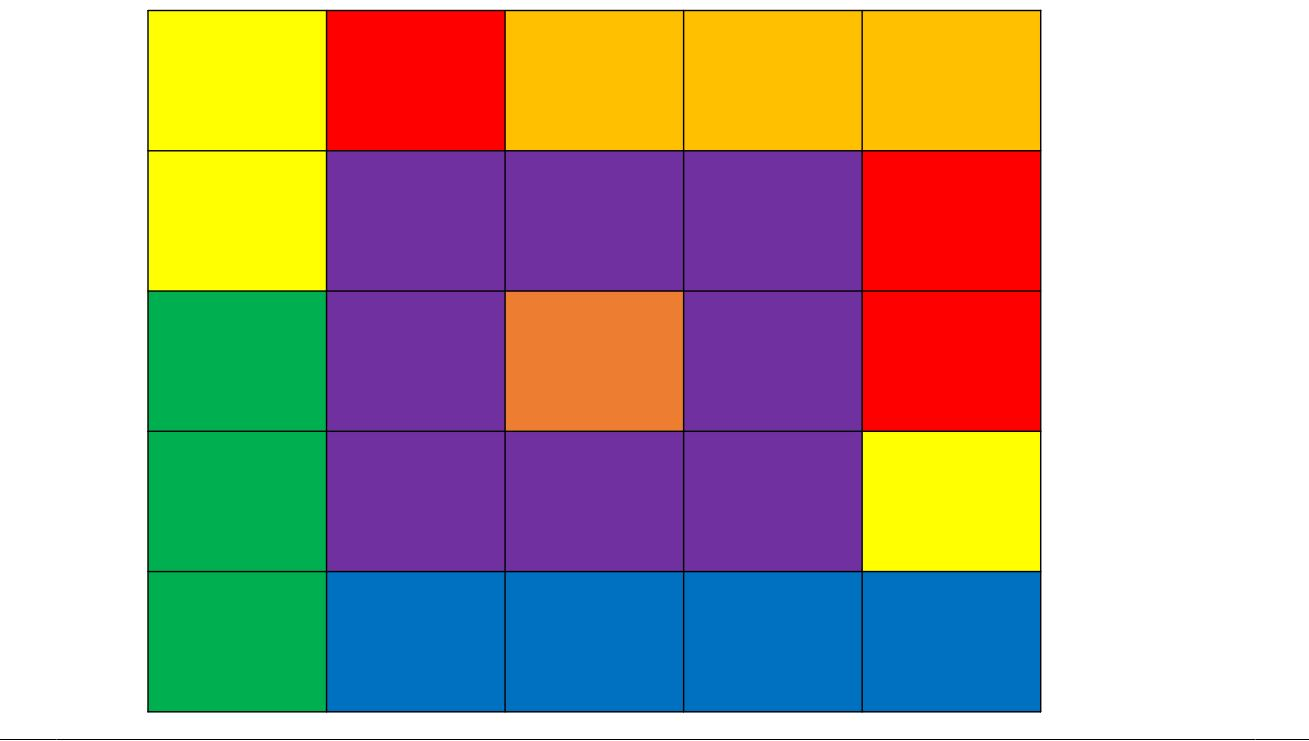
\includegraphics[width=1.0\textwidth]{Figures/example_figure2.JPG}
    \caption{Example figure 2.}
    \label{figexample_figure2}
    \end{figure}
    It has been shown that it is i good thing \citep{example_reference2}. 
    
    \section{Name of section 2}
    %Bare for å generere noe tekst for å se hvordan det ser ut:
    \lipsum[1]\\
    This is a good measure \citep{example_reference3}.\\ \\
    
    
    \section{Name of section 3}
    %Bare for å generere noe tekst for å se hvordan det ser ut:
    \lipsum[1]
    
%%%%%%%%%%%%%%%%%%%%%%%%%%%%%%%%%%%%%%%%%%%%%%%%%%%%%%%%%%%%%%%
\biblio
\cleardoublepage
\end{document}